\chapter{ Экспериментальный раздел}
Данный раздел посвящен тестированию и исследованию трех реализованных алгоримтов: алгоритмам Левенштейна, Дамерау -- Левенштейна и рекурсивной реализации Левенштейна.

\section{ Примеры работы}
Алгоритм Левенштейна:

\begin{lstlisting}
Input s1: OTAPA
Input s2: TAPTAP

0 1 2 3 4 5 6
1 1 2 3 4 5 6
2 1 2 3 3 4 5
3 2 1 2 3 3 4
4 3 2 1 2 3 3
5 4 3 2 2 2 3
\end{lstlisting}

\begin{lstlisting}
Input s1: MGTU
Input s2: MTGU

0 1 2 3 4
1 0 1 2 3
2 1 1 1 2
3 2 1 2 2
4 3 2 2 2
\end{lstlisting}

Алгоритм Дамерау -- Левенштейна:

\begin{lstlisting}
Input s1: MGTU
Input s2: MTGU

0 1 2 3 4
1 0 1 2 3
2 1 1 1 2
3 2 1 1 2
4 3 2 2 1
\end{lstlisting}

\begin{lstlisting}
Input s1: KNUTH
Input s2: TANENBAUM

0 1 2 3 4 5 6 7 8 9
1 1 2 3 4 5 6 7 8 9
2 2 2 2 3 4 5 6 7 8
3 3 3 3 3 4 5 6 6 7
4 3 4 4 4 4 5 6 7 7
5 4 4 5 5 5 5 6 7 8
\end{lstlisting}

Алгоритм Левенштейна(Рекурсивный):

\begin{lstlisting}
Input s1: MGTU
Input s2: MTGU
Length is : 2
\end{lstlisting}

\begin{lstlisting}
Input s1: OTAPA
Input s2: TAPTAP
Length is : 3
\end{lstlisting}

\section{ Постановка эксперимента}
Эксперимент проводится в виде поочередного запуска программы, в которой находится расстояние между строками, подающимися на вход. Длина строк варьируется от 100 до 1000 с шагом 100, при чем каждую итерацию призводится 100 кратный пересчет расстояния с одинаковыми данными для частоты эксперимента. Далее находится среднее значение времени для каждой подсчитанной части. Так как частота вызовов рекурсивной функции становится большой начиная со строк длинной более 6 символов, очень сложно реализовать эксперемент с длинной строк от 100 до 1000 на этом алгоритме, так как вычислительная машина, на которой проводится эксперимент не достаточно мощная. Поэтому для рекурсивной реализации будет проводиться эксперимент с длинной строк от 1 до 10 с шагом 1. 

\section{ Сравнительный анализ на материале экспериментальных данных}

На рисунке \ref{fig:exp1} представлен первый эксперемент, на котором наглядно продемонстрированно изменение времени двух алгоритмов: Дамерау -- Левенштейна и Левенштейна. Рекурсивная реализация отсутствует(причины представлены во втором эксперементе \ref{fig:exp2}). Здесь можно заметить, что реализация Дамерау -- Левенштейна начинает значительно медленнее работать, чем реализация Левенштейна. 

\begin{figure}[ht!]
    \centering{
        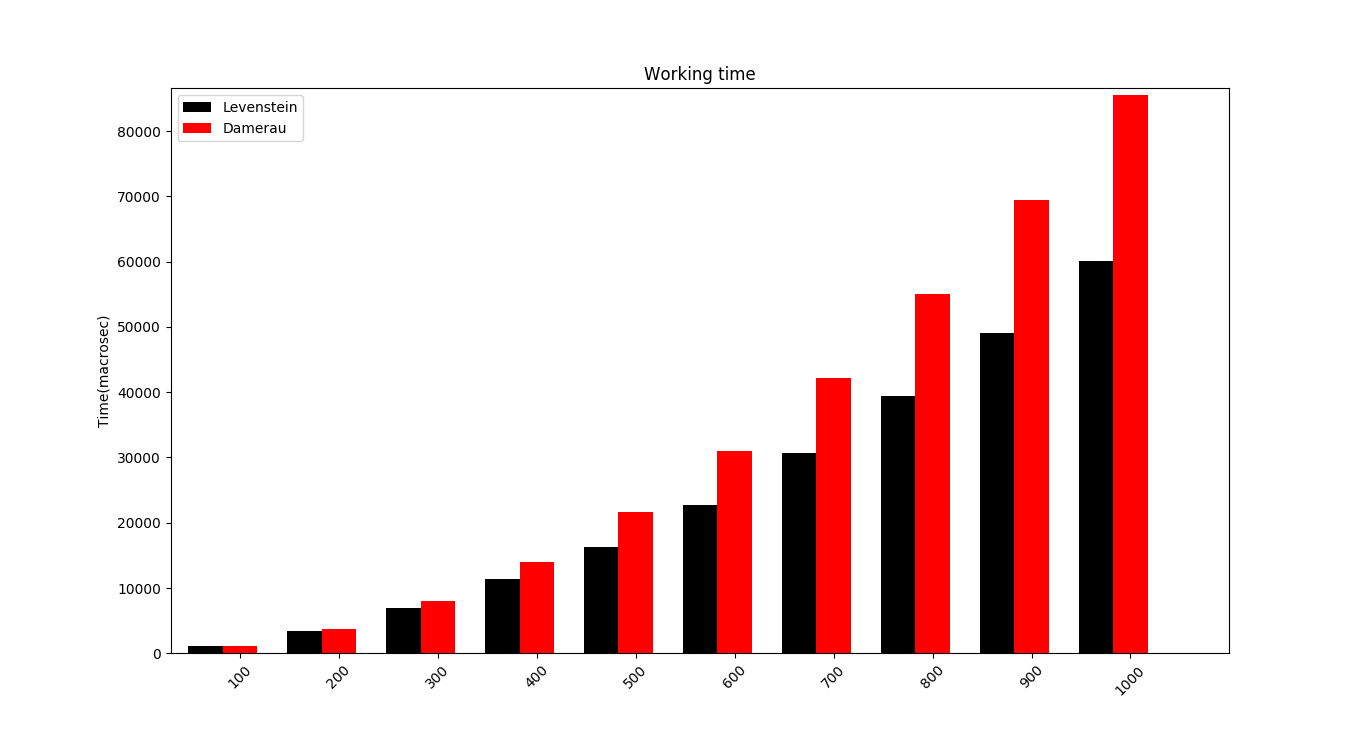
\includegraphics[width=1\textwidth]{img/exp1.png}
        \caption{ Эксперемент первый, демонстрация различия времени для алгоритмов Левенштейна и Дамерау -- Левенштейна}
        \label{fig:exp1}
    }
\end{figure}

Рисунок \ref{fig:exp2} отображает второй эксперимент, в котором уже в рассчет брался рекурсивный метод Левенштейна. Он не был включен в первый, потому что время, затраченное на нахождение расстояния резко подскакивает уже на длиннах строк равных 5. Чем больше значение, тем больше время(оно начинает повышаться в несколько раз). Если обратить внимание на Левенштейна и Дамерау -- Левенштейна, можно заметить, что алгоритм Левенштейна работает медленнее Дамерау -- Левенштейна с маленькими строками, но в первом эксперименте наглядно показано, что на больших строках, Левенштейн показывает большую эффективность.

\begin{figure}[ht!]
    \centering{
        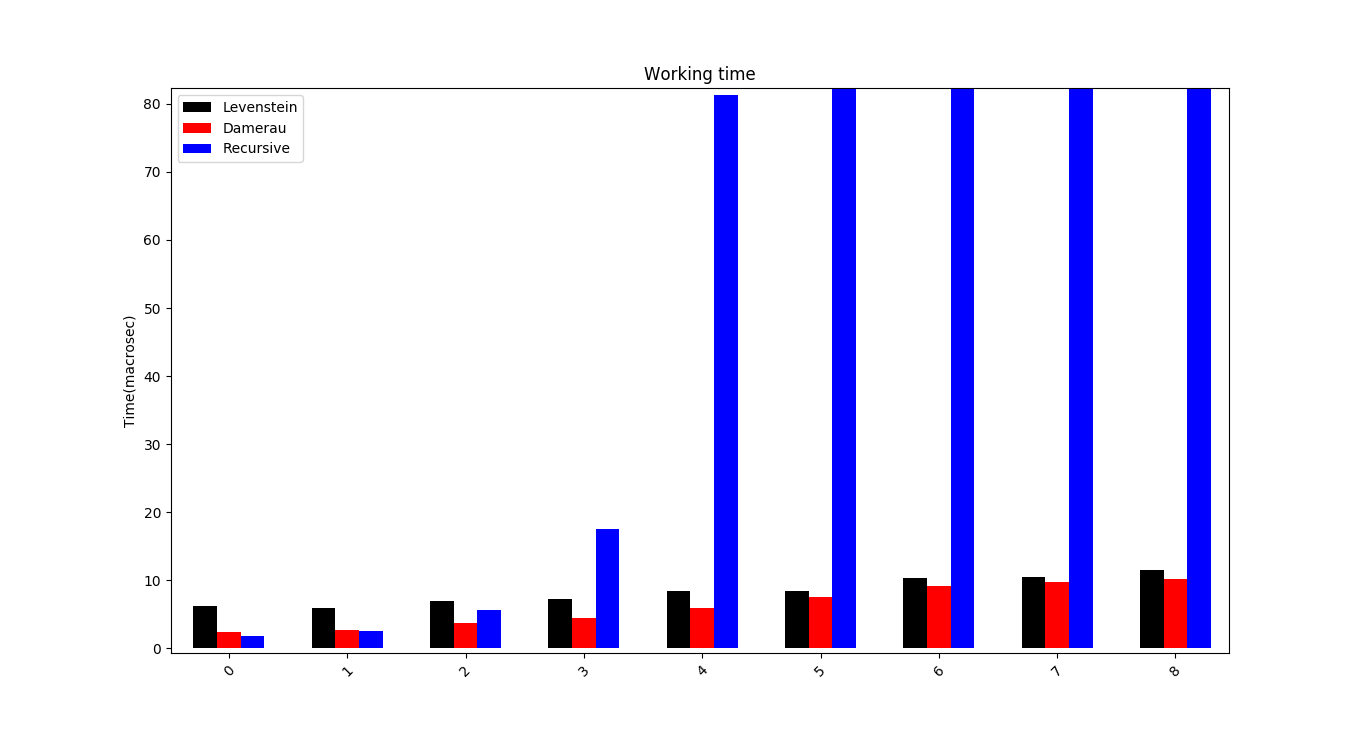
\includegraphics[width=1\textwidth]{img/exp2.png}
        \caption{ Эксперемент второй, демонстрация различия времени для алгоритмов Левенштейна и Дамерау -- Левенштейна и рекурсивной реализации Левенштейна}
        \label{fig:exp2}
    }
\end{figure}

Из-за большого количества рекурсивных запросов, метод работает медленно и чем больше длина слова, тем больше вызовов производится:

\begin{lstlisting}
 Input s1: OTAPA
 Input s2: TAPTAP
Length is : 3
function called 5479 times
\end{lstlisting}

\begin{lstlisting}
 Input s1: FLEICHE
 Input s2: EUROPA
Length is : 6
function called 29737 times
\end{lstlisting}

\begin{lstlisting}
 Input s1: ENTSCHULDIGUNG
 Input s2: EINWAGEN
Length is : 11
function called 21820057 times
\end{lstlisting}

В листинге \ref{list:rec} представлено рекурсивное дерево на примере поиска редакционного расстояния между строками MGT, MTG. Производится очень много повторяющихся вызовов, которые каждый раз пересчитываются.

\begin{lstlisting}[caption={ Recursive tree example MGT, MTG},
                   captionpos=b,
                   label={list:rec}]
function called 94 times
(MGT, MTG)
 `--(MG, MT)
 |   `--(M, M)
 |   |   `--(, )
 |   |   `--(M, )
 |   |   `--(, M)
 |   `--(MG, M)
 |   |   `--(M, )
 |   |   `--(MG, )
 |   |   `--(M, M)
 |   |       `--(, )
 |   |       `--(M, )
 |   |       `--(, M)
 |   `--(M, MT)
 |       `--(, M)
 |       `--(M, M)
 |       |   `--(, )
 |       |   `--(M, )
 |       |   `--(, M)
 |       `--(, MT)
 `--(MGT, MT)
 |   `--(MG, M)
 |   |   `--(M, )
 |   |   `--(MG, )
 |   |   `--(M, M)
 |   |       `--(, )
 |   |       `--(M, )
 |   |       `--(, M)
 |   `--(MGT, M)
 |   |   `--(MG, )
 |   |   `--(MGT, )
 |   |   `--(MG, M)
 |   |       `--(M, )
 |   |       `--(MG, )
 |   |       `--(M, M)
 |   |           `--(, )
 |   |           `--(M, )
 |   |           `--(, M)
 |   `--(MG, MT)
 |       `--(M, M)
 |       |   `--(, )
 |       |   `--(M, )
 |       |   `--(, M)
 |       `--(MG, M)
 |       |   `--(M, )
 |       |   `--(MG, )
 |       |   `--(M, M)
 |       |       `--(, )
 |       |       `--(M, )
 |       |       `--(, M)
 |       `--(M, MT)
 |           `--(, M)
 |           `--(M, M)
 |           |   `--(, )
 |           |   `--(M, )
 |           |   `--(, M)
 |           `--(, MT)
 `--(MG, MTG)
     `--(M, MT)
     |   `--(, M)
     |   `--(M, M)
     |   |   `--(, )
     |   |   `--(M, )
     |   |   `--(, M)
     |   `--(, MT)
     `--(MG, MT)
     |   `--(M, M)
     |   |   `--(, )
     |   |   `--(M, )
     |   |   `--(, M)
     |   `--(MG, M)
     |   |   `--(M, )
     |   |   `--(MG, )
     |   |   `--(M, M)
     |   |       `--(, )
     |   |       `--(M, )
     |   |       `--(, M)
     |   `--(M, MT)
     |       `--(, M)
     |       `--(M, M)
     |       |   `--(, )
     |       |   `--(M, )
     |       |   `--(, M)
     |       `--(, MT)
     `--(M, MTG)
         `--(, MT)
         `--(M, MT)
         |   `--(, M)
         |   `--(M, M)
         |   |   `--(, )
         |   |   `--(M, )
         |   |   `--(, M)
         |   `--(, MT)
         `--(, MTG)
\end{lstlisting}


Из диаграм наглядно видно, что алгоритм Левенштейна гораздо эффективнее его рекурсивной реализации, при работе с большим объемом данных рекурсивная реализация просто никуда не годится. 

Память в программах была использована эффективно, не было никаких утечек:

Рекурсивная реализация алгоритма Левенштейна(valgrind):
\begin{lstlisting}
==21413== HEAP SUMMARY:
==21413==     in use at exit: 0 bytes in 0 blocks
==21413==   total heap usage: 2 allocs, 2 frees, 2,048 bytes allocated
\end{lstlisting}

Алгоритм Левенштйена(valgrind):
\begin{lstlisting}
==21460== HEAP SUMMARY:
==21460==     in use at exit: 0 bytes in 0 blocks
==21460==   total heap usage: 2 allocs, 2 frees, 2,048 bytes allocated
\end{lstlisting}

Алгоритм Дамерау -- Левенштейна(valgrind):
\begin{lstlisting}
==21489== HEAP SUMMARY:
==21489==     in use at exit: 0 bytes in 0 blocks
==21489==   total heap usage: 2 allocs, 2 frees, 2,048 bytes allocated
\end{lstlisting}
